\documentclass[12pt,a4paper]{report}

% ==============================================================================
% 1. PACKAGES FONDAMENTAUX & CONFIGURATION TYPOGRAPHIQUE
% ==============================================================================
\usepackage[utf8]{inputenc}
\usepackage[T1]{fontenc}
\usepackage[french]{babel}
\usepackage{lmodern}
\usepackage{microtype}

% Marges conformes aux standards académiques
\usepackage[top=2.5cm, bottom=2.5cm, left=2.5cm, right=2.5cm]{geometry}

% Graphiques, figures et positionnement
\usepackage{graphicx}
\usepackage{float}
\usepackage{subcaption}

% Tableaux professionnels
\usepackage{booktabs}
\usepackage{tabularx}
\usepackage{array}
\usepackage{multirow}

% Formules mathématiques et symboles
\usepackage{amsmath}
\usepackage{amssymb}

% Couleurs personnalisées (Palette professionnelle CyberSécurité)
\usepackage{xcolor}
\definecolor{ensetblue}{RGB}{16, 44, 87}
\definecolor{navyaccent}{RGB}{20, 80, 160}
\definecolor{darkslate}{RGB}{30, 41, 59}
\definecolor{codegray}{RGB}{246, 248, 251}
\definecolor{bordergray}{RGB}{218, 224, 233}
\definecolor{commentgreen}{RGB}{34, 139, 34}
\definecolor{stringred}{RGB}{178, 34, 34}
\definecolor{keywordblue}{RGB}{0, 51, 153}
\definecolor{terminalbg}{RGB}{15, 23, 42}
\definecolor{terminaltext}{RGB}{226, 232, 240}

% Encadrés élégants (tcolorbox)
\usepackage[most]{tcolorbox}
\newtcolorbox{infobox}[1][]{
    enhanced,
    colback=codegray,
    colframe=navyaccent,
    fonttitle=\bfseries\color{white},
    coltitle=white,
    colbacktitle=navyaccent,
    attach boxed title to top left={yshift=-2mm, xshift=4mm},
    boxed title style={boxrule=0.5mm},
    arc=2mm,
    #1
}

\newtcolorbox{terminalbox}[1][]{
    enhanced,
    colback=terminalbg,
    colframe=darkslate,
    fonttitle=\bfseries\color{terminaltext},
    coltitle=terminaltext,
    arc=2mm,
    #1
}

% En-têtes et pieds de page personnalisés
\usepackage{fancyhdr}
\pagestyle{fancy}
\fancyhf{}
\fancyhead[L]{\small\color{darkslate}\textit{ENSET Mohammedia -- Confiance Numérique}}
\fancyhead[R]{\small\color{darkslate}\textit{TP PKI : CCN\_PKI (MVP)}}
\fancyfoot[L]{\small\color{darkslate}Option 2 : Développement d'un MVP PKI}
\fancyfoot[R]{\thepage}
\renewcommand{\headrulewidth}{0.4pt}
\renewcommand{\footrulewidth}{0.4pt}

% Configuration des titres de section
\usepackage{titlesec}
\titleformat{\chapter}[display]
  {\normalfont\bfseries\color{ensetblue}}
  {\filleft\Huge\thechapter}
  {1ex}
  {\titlerule\vspace{1ex}\huge}
\titleformat{\section}
  {\normalfont\Large\bfseries\color{ensetblue}}{\thesection}{1em}{}
\titleformat{\subsection}
  {\normalfont\large\bfseries\color{navyaccent}}{\thesubsection}{1em}{}
\titleformat{\subsubsection}
  {\normalfont\normalsize\bfseries\color{darkslate}}{\thesubsubsection}{1em}{}

% Configuration du code source (listings)
\usepackage{listings}
\lstset{
    backgroundcolor=\color{codegray},
    commentstyle=\color{commentgreen}\itshape,
    keywordstyle=\color{keywordblue}\bfseries,
    numberstyle=\tiny\color{gray},
    stringstyle=\color{stringred},
    basicstyle=\ttfamily\footnotesize,
    breakatwhitespace=false,
    breaklines=true,
    captionpos=b,
    keepspaces=true,
    numbers=left,
    numbersep=7pt,
    showspaces=false,
    showstringspaces=false,
    showtabs=false,
    tabsize=2,
    frame=single,
    rulecolor=\color{bordergray},
    xleftmargin=10pt,
    framexleftmargin=5pt
}

% Hyperliens cliquables et métadonnées PDF
\usepackage{hyperref}
\hypersetup{
    colorlinks=true,
    linkcolor=ensetblue,
    citecolor=navyaccent,
    urlcolor=navyaccent,
    pdfauthor={Groupe ENSET Mohammedia},
    pdftitle={Rapport TP PKI : Conception d'une Infrastructure à Clés Publiques (CCN_PKI)},
    pdfsubject={Confiance Numérique et Accès Biométrique},
    pdfkeywords={PKI, X.509, CRL, RFC 5280, Spring Boot, Bouncy Castle, OpenSSL, Docker}
}

% ==============================================================================
% 2. DOCUMENT PRINCIPAL
% ==============================================================================
\begin{document}

% ------------------------------------------------------------------------------
% PAGE DE GARDE INSTITUTIONNELLE
% ------------------------------------------------------------------------------
\begin{titlepage}
    \begin{center}
        % En-tête institutionnel
        {\large \textbf{UNIVERSITÉ HASSAN II DE CASABLANCA}}\\[0.2cm]
        {\large \textbf{ÉCOLE NORMALE SUPÉRIEURE DE L'ENSEIGNEMENT TECHNIQUE}}\\[0.1cm]
        {\Large \textbf{ENSET MOHAMMEDIA}}\\[0.2cm]
        {\normalsize \textit{Département Mathématiques et Informatique}}\\[0.1cm]
        {\normalsize \textit{Filière : Master / Cycle d'Ingénieur -- Génie Informatique \& CyberSécurité}}\\[0.6cm]

        % Règle de séparation élégante
        \rule{0.75\textwidth}{1.2pt}

        \vspace{0.8cm}

        % Cadre du Titre Principal
        \begin{tcolorbox}[colback=ensetblue!5, colframe=ensetblue, width=\textwidth, arc=3mm, boxrule=1.5pt]
            \centering
            \vspace{0.3cm}
            {\Large \textbf{RAPPORT DE TRAVAUX PRATIQUES}}\\[0.3cm]
            {\LARGE \textbf{Conception d'une Infrastructure à Clés Publiques}}\\[0.2cm]
            {\Large \textbf{Module : Confiance Numérique et Accès Biométrique}}\\[0.3cm]
            \rule{0.85\textwidth}{0.8pt}\\[0.3cm]
            {\large \textbf{Option 2 : Développement d'un MVP PKI (« CCN\_PKI »)}}\\[0.1cm]
            {\small Implémentation complète conforme RFC 5280 (X.509 v3, CRL v2, Spring Boot \& Docker)}
            \vspace{0.3cm}
        \end{tcolorbox}

        \vspace{1.2cm}

        % Tableau des Membres et Encadrant
        \begin{minipage}[t]{0.52\textwidth}
            \textbf{Réalisé par le Groupe (4 Étudiants) :}\\[0.3cm]
            \begin{itemize}
                \item \textbf{Étudiant 1 : } Nom \& Prénom (\texttt{CNE / Apogée})
                \item \textbf{Étudiant 2 : } Nom \& Prénom (\texttt{CNE / Apogée})
                \item \textbf{Étudiant 3 : } Nom \& Prénom (\texttt{CNE / Apogée})
                \item \textbf{Étudiant 4 : } Nom \& Prénom (\texttt{CNE / Apogée})
                % TODO: Compléter avec les noms, prénoms et matricules officiels du groupe
            \end{itemize}
        \end{minipage}
        \hfill
        \begin{minipage}[t]{0.42\textwidth}
            \begin{flushright}
                \textbf{Sous la direction de :}\\[0.3cm]
                \textbf{Pr. [Nom du Professeur]}\\[0.1cm]
                {\small Enseignant-Chercheur}\\[0.1cm]
                {\small ENSET Mohammedia}\\[1.5cm]
                \textbf{Année Universitaire :}\\[0.1cm]
                2025 -- 2026
            \end{flushright}
        \end{minipage}

        \vfill
        {\footnotesize \textbf{Dépôt GitHub du Projet :} \url{https://github.com/AsaadFethallah/CCN_PKI}}
    \end{center}
\end{titlepage}

% ------------------------------------------------------------------------------
% PAGES LIMINAIRES : RÉSUMÉ, TABLES DES MATIÈRES & FIGURES
% ------------------------------------------------------------------------------
\pagenumbering{roman}

\chapter*{Résumé Exécutif}
Dans le cadre du module \textit{Confiance Numérique et Accès Biométrique} dispensé à l'ENSET Mohammedia, ce projet présente la conception, l'implémentation industrielle et la validation d'une \textbf{Infrastructure à Clés Publiques minimale mais complète (MVP)}, baptisée \textbf{CCN\_PKI}. 

Conformément au cahier des charges de l'\textbf{Option 2}, nous avons développé une autorité de certification racine (\textit{Root CA}) auto-signée reposant sur l'écosystème \textbf{Spring Boot 3} et le moteur cryptographique de référence \textbf{Bouncy Castle 1.79}. La solution offre l'émission de certificats d'entité finale en mode direct (génération de biclé et export d'archives sécurisées PKCS\#12) ainsi qu'en mode CSR (\textit{PKCS\#10 Certificate Signing Request}) avec vérification rigoureuse de la preuve de possession. 

Le système intègre la gestion dynamique des révocations selon la \textbf{RFC 5280} avec publication de Listes de Révocation de Certificats (\textbf{CRL X.509 v2}) signées par l'autorité. Un moteur de validation cryptographique interne permet l'inspection détaillée des certificats, complété par une intégration certifiée et vérifiée avec la suite d'audit international \textbf{OpenSSL CLI}. L'ensemble de la solution est conteneurisé sous forme d'image légère Alpine Linux orchestrée par \textbf{Docker Compose}, garantissant une reproductibilité et une persistance sans faille.

\vspace{0.8cm}
\noindent \textbf{Mots-clés :} PKI, Root CA, Certificat X.509 v3, CRL v2, RFC 5280, Bouncy Castle, Spring Boot, OpenSSL, Docker.

\vspace{1cm}
\tableofcontents
\listoffigures
\listoftables

\clearpage
\pagenumbering{arabic}

% ==============================================================================
% CHAPITRE 1 : CONTEXTE ET OBJECTIFS DU PROJET
% ==============================================================================
\chapter{Contexte et Objectifs du Projet}

\section{Introduction à la Confiance Numérique et aux PKI}
Dans un cyber-espace décentralisé et intrinsèquement non sécurisé, la cryptographie asymétrique résout le problème de la confidentialité mais laisse en suspens la question cruciale de l'authenticité : \textit{Comment avoir l'assurance mathématique qu'une clé publique appartient bien à l'entité qui la revendique ?}

L'Infrastructure à Clés Publiques (\textbf{PKI} -- \textit{Public Key Infrastructure}) constitue la réponse universelle à cette problématique. En liant formellement une identité vérifiée à un couple de clés asymétriques à travers un document numérique infalsifiable -- le \textbf{certificat X.509} -- l'Autorité de Certification (\textbf{CA}) s'érige en tiers de confiance incontestable.

\section{Justification du Choix du Projet (Option 2 : Développement MVP)}
Le sujet du travail pratique proposé par l'ENSET Mohammedia présentait deux alternatives :
\begin{enumerate}
    \item \textbf{Option 1 :} L'analyse et l'audit d'une solution PKI open source existante (telle qu'EJBCA, OpenXPKI ou Smallstep).
    \item \textbf{Option 2 :} Le développement \textit{from scratch} d'un MVP (\textit{Minimum Viable Product}) d'une PKI implémentant une Root CA, la signature de certificats et l'émission d'une CRL conforme.
\end{enumerate}

Notre groupe a fait le choix ambitieux de l'\textbf{Option 2}. Ce choix se justifie par la volonté d'acquérir une compréhension intime et opérationnelle des primitives cryptographiques, des structures de données ASN.1, de l'encodage DER/PEM et de la mécanique de signature et de révocation définie par les normes internationales de l'IETF.

\section{Cahier des Charges et Objectifs Réalisés}
Le système développé, intitulé \textbf{CCN\_PKI}, satisfait l'intégralité des spécifications requises ainsi que plusieurs valorisations d'ingénierie :
\begin{itemize}
    \item \textbf{Autorité Racine (Root CA) :} Génération d'une biclé RSA 4096 bits et création d'un certificat auto-signé X.509 v3 avec extensions critiques obligatoires.
    \item \textbf{Émission Multi-Profils :} Support de certificats pour l'authentification client (mTLS), serveurs web (avec extensions SAN) et signature de code.
    \item \textbf{Support des Demandes CSR (PKCS\#10) :} Validation de la signature interne du client (\textit{Proof of Possession}) et émission sans divulgation de la clé privée cliente.
    \item \textbf{Gestion des Révocations (CRL v2) :} Révocation granulaire selon les motifs de la RFC 5280 et publication immédiate d'une CRL signée.
    \item \textbf{Double Mécanisme de Validation :} Moteur applicatif natif et vérification standardisée via OpenSSL CLI (\texttt{openssl verify -crl\_check}).
    \item \textbf{Conteneurisation et Déploiement :} Automatisation multi-stage sous Docker Compose pour un démarrage en un clic.
\end{itemize}

% ==============================================================================
% CHAPITRE 2 : ARCHITECTURE GÉNÉRALE DU SYSTÈME
% ==============================================================================
\chapter{Architecture Générale du Système}

\section{Découpage Modulaire et Architecture à Cinq Niveaux}
Le système \textbf{CCN\_PKI} est architecturé selon un modèle robuste à cinq niveaux horizontaux (\textit{Tiered Architecture}), garantissant une séparation étanche des responsabilités entre les consommateurs de services, l'interface graphique, la logique métier de sécurité, les moteurs cryptographiques de bas niveau et la persistance des données. 

La figure~\ref{fig:architecture_systeme} illustre l'organisation des composants, leurs interfaces de communication ainsi que les flux de données traversant le conteneur Docker.

\begin{figure}[H]
    \centering
    % TODO : Ajouter la capture d'écran ici
    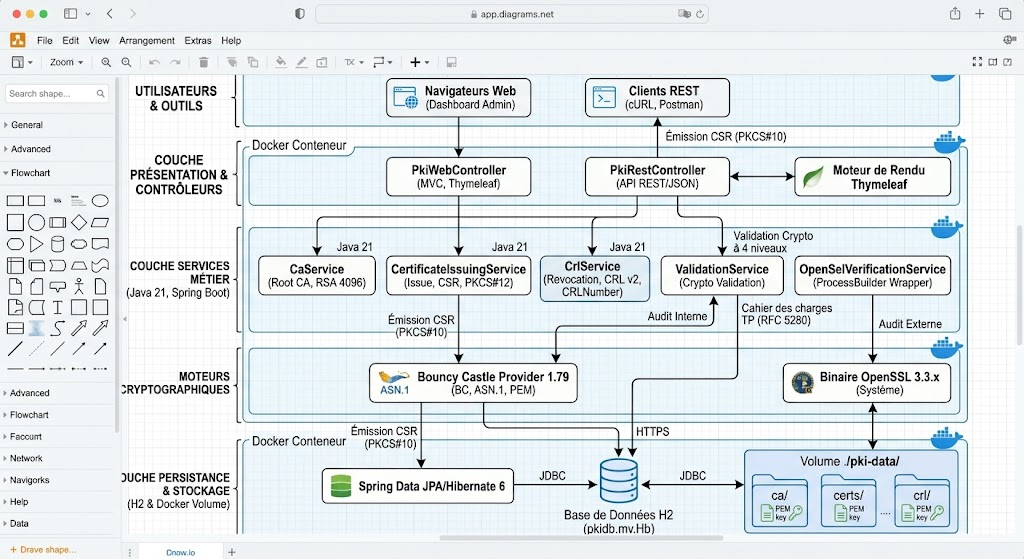
\includegraphics[width=\textwidth]{images/ec11dd04-7423-4542-8641-67e67307af10.jpeg}
    \caption{Architecture technique à 5 niveaux et flux de données de la solution CCN\_PKI}
    \label{fig:architecture_systeme}
\end{figure}

\subsection{Description Détaillée des Cinq Niveaux}

\begin{enumerate}
    \item \textbf{Niveau 1 : Utilisateurs \& Outils (Environnement Client) :}
    \begin{itemize}
        \item \textbf{Navigateurs Web (Dashboard Admin) :} Permet aux opérateurs de sécurité et aux étudiants d'interagir graphiquement avec l'infrastructure (visualisation de la Root CA, formulaires d'émission directe ou CSR, consultation de la liste des certificats, révocation et tableau de bord de métriques).
        \item \textbf{Clients REST (cURL, Postman, Scripts d'automatisation) :} Consomment directement les points d'accès HTTP RESTful pour soumettre des demandes de signature CSR (\textit{PKCS\#10}) ou intégrer les opérations PKI dans des pipelines CI/CD et des scripts d'administration.
    \end{itemize}

    \item \textbf{Niveau 2 : Couche Présentation \& Contrôleurs (Docker Conteneur) :}
    \begin{itemize}
        \item \textbf{PkiWebController :} Contrôleur Spring MVC assurant le routage des requêtes web utilisateur et l'injection des modèles dans les gabarits de présentation.
        \item \textbf{PkiRestController :} Contrôleur d'API exposant les endpoints RESTful au format JSON, PEM et binaire DER (\texttt{/api/pki/*}).
        \item \textbf{Moteur de Rendu Thymeleaf :} Moteur de templating côté serveur générant dynamiquement les vues HTML5/CSS3 adaptées au thème CyberSécurité.
    \end{itemize}

    \item \textbf{Niveau 3 : Couche Services Métier (Java 21 LTS / Spring Boot 3) :}
    \begin{itemize}
        \item \textbf{CaService :} Supervise le cycle de vie complet de l'Autorité Racine auto-signée (Root CA, RSA 4096 bits), l'accès sécurisé à la clé privée de l'autorité et la persistance sur le système de fichiers.
        \item \textbf{CertificateIssuingService :} Gère l'émission centralisée directe (génération de biclé et confection de trousseaux PKCS\#12 chiffrés) ainsi que la signature décentralisée des demandes CSR (PKCS\#10) avec validation formelle de la preuve de possession cryptographique (\textit{Proof of Possession}).
        \item \textbf{CrlService :} Traite les demandes de révocation selon les motifs RFC 5280, pilote l'incrémentation séquentielle du numéro de CRL (\texttt{CRLNumber}) et orchestre la publication dynamique de la CRL X.509 v2.
        \item \textbf{ValidationService :} Moteur d'audit cryptographique interne exécutant une vérification séquentielle à 4 niveaux (syntaxe ASN.1, admissibilité temporelle, intégrité mathématique de la signature de la CA, et contrôle d'absence dans la CRL active).
        \item \textbf{OpenSslVerificationService :} Wrapper exploitant l'API \texttt{ProcessBuilder} pour invoquer directement le binaire système OpenSSL et générer des rapports de conformité indépendants.
    \end{itemize}

    \item \textbf{Niveau 4 : Moteurs Cryptographiques de Bas Niveau :}
    \begin{itemize}
        \item \textbf{Bouncy Castle Provider 1.79 (Provider « BC ») :} Cœur cryptographique de l'application, fournissant l'implémentation agréée des primitives de chiffrement asymétrique RSA, de hachage SHA-256, de construction des structures de données ASN.1 et d'encodage/décodage PEM.
        \item \textbf{Binaire Système OpenSSL 3.3.x :} Présent nativement au sein de l'image Alpine Linux pour réaliser les audits externes officiels (\texttt{openssl verify -crl\_check}) sans nécessiter d'installation préalable sur le poste hôte.
    \end{itemize}

    \item \textbf{Niveau 5 : Couche Persistance \& Stockage (H2 \& Volume Docker) :}
    \begin{itemize}
        \item \textbf{Spring Data JPA / Hibernate 6 :} Couche d'abstraction et d'accès aux données simplifiant les opérations transactionnelles CRUD sur les entités de sécurité.
        \item \textbf{Base de Données Relationnelle H2 (pkidb.mv.db) :} Moteur de base de données embarqué rapide et persistant, accessible via protocole JDBC, hébergeant les tables \texttt{CA\_ENTITY}, \texttt{CERTIFICATES} et \texttt{CRL\_ENTITY}.
        \item \textbf{Volume Docker Persistant (\texttt{./pki-data/}) :} Montage hôte/conteneur garantissant l'intégrité physique et la pérennité des artefacts cryptographiques à travers les redémarrages :
        \begin{itemize}
            \item \texttt{pki-data/ca/} : Clés et certificat de l'Autorité Racine (\texttt{rootCA.crt}, \texttt{rootCA.key}).
            \item \texttt{pki-data/certs/} : Certificats d'entité finale (\texttt{.crt}), clés privées associées (\texttt{.key}) et archives sécurisées (\texttt{.p12}).
            \item \texttt{pki-data/crl/} : Listes de révocation actives sous forme textuelle PEM (\texttt{crl.pem}) et binaire ASN.1 DER (\texttt{crl.crl}).
        \end{itemize}
    \end{itemize}
\end{enumerate}

\subsection{Trajectoire et Flux de Données Critiques}
L'architecture illustrée met en exergue trois flux cardinaux :
\begin{itemize}
    \item \textbf{Flux d'Émission via CSR (PKCS\#10) :} Le client soumet sa demande au format PEM vers le \texttt{PkiRestController}. La requête est transmise au \texttt{CertificateIssuingService}, qui sollicite \textbf{Bouncy Castle} pour vérifier la validité de la signature de la CSR. Une fois la preuve de possession attestée, le service forge le certificat X.509 v3, l'authentifie avec la clé privée de la Root CA, le persiste en base H2 et exporte le fichier \texttt{.crt} sur le volume disque avant restitution au client.
    \item \textbf{Flux d'Audit Interne (Validation à 4 Niveaux) :} Le \texttt{ValidationService} reçoit le certificat à examiner, analyse sa syntaxe ASN.1, vérifie que la date courante s'inscrit dans la période d'admissibilité, déchiffre la signature grâce à la clé publique de la CA, et s'assure auprès du \texttt{CrlService} que le numéro de série ne figure pas dans la CRL active.
    \item \textbf{Flux d'Audit Externe OpenSSL :} L'\texttt{OpenSslVerificationService} invoque en sous-processus sécurisé le binaire \texttt{/usr/bin/openssl} en lui injectant les fichiers \texttt{rootCA.pem}, \texttt{crl.pem} et le certificat cible avec le drapeau strict \texttt{-crl\_check}, recueillant les codes de diagnostic universels (tel que l'\textit{Erreur 23}).
\end{itemize}

\section{Organisation Détaillée des Paquetages et Classes}
Le tableau~\ref{tab:classes_projet} synthétise le rôle des classes maîtresses développées dans le projet.

\begin{table}[H]
\centering
\small
\begin{tabularx}{\textwidth}{l p{5.5cm} X}
\toprule
\textbf{Paquetage} & \textbf{Classe / Interface} & \textbf{Rôle Fonctionnel et Cryptographique} \\
\midrule
\texttt{service} & \texttt{CaService.java} & Cycle de vie de la Root CA, biclé RSA 4096, auto-signature et synchronisation disque. \\
\addlinespace
\texttt{service} & \texttt{CertificateIssuingService.java} & Émission X.509 v3 directe, validation CSR PKCS\#10 et injection d'extensions RFC 5280. \\
\addlinespace
\texttt{service} & \texttt{CrlService.java} & Enregistrement des motifs RFC 5280, génération et signature de la CRL X.509 v2. \\
\addlinespace
\texttt{service} & \texttt{ValidationService.java} & Moteur d'audit 4 étapes : format, temporalité, signature CA et contrôle CRL. \\
\addlinespace
\texttt{service} & \texttt{OpenSslVerificationService.java} & Invocation et exécution automatisée du binaire OpenSSL système pour tests croisés. \\
\addlinespace
\texttt{util} & \texttt{PemUtils.java} & Sérialisation / désérialisation PEM, empreintes SHA-256 et confection de trousseaux PKCS\#12. \\
\addlinespace
\texttt{controller} & \texttt{PkiRestController.java} & Points de terminaison RESTful JSON, PEM et DER pour l'automatisation système. \\
\addlinespace
\texttt{controller} & \texttt{PkiWebController.java} & Routage MVC et alimentation des vues interactives du tableau de bord. \\
\bottomrule
\end{tabularx}
\caption{Cartographie des classes et services du projet CCN\_PKI}
\label{tab:classes_projet}
\end{table}

\section{Étude Approfondie de la Bibliothèque Cryptographique Bouncy Castle 1.79}

\subsection{Présentation et Rôle dans l'Architecture CCN\_PKI}
Pour concrétiser les exigences d'une Autorité Racine et satisfaire l'ensemble des primitives requises par la RFC 5280, le choix d'un fournisseur cryptographique de premier ordre était capital. Notre implémentation repose intégralement sur la suite logicielle de référence mondiale : \textbf{The Legion of the Bouncy Castle} (version \textbf{1.79}), à travers ses deux modules complémentaires :
\begin{enumerate}
    \item \textbf{\texttt{bcprov-jdk18on} (Bouncy Castle Provider) :} Fournit les implémentations algorithmiques de bas niveau compatibles avec l'architecture de sécurité Java (\textit{Java Cryptography Extension - JCE}). Il prend en charge la génération de nombres pseudo-aléatoires sécurisés (\texttt{SecureRandom}), le chiffrement asymétrique RSA (clés 2048 et 4096 bits), le hachage sécurisé SHA-256 et le déchiffrement des conteneurs protégés.
    \item \textbf{\texttt{bcpkix-jdk18on} (PKIX / CMS / EAC / PKCS APIs) :} Fournit les structures de haut niveau dédiées aux infrastructures à clés publiques, notamment la manipulation de la syntaxe ASN.1, les générateurs de certificats X.509 v3 (\texttt{JcaX509v3CertificateBuilder}), les générateurs de listes de révocation v2 (\texttt{X509v2CRLBuilder}) et l'analyseur de requêtes CSR (\texttt{PKCS10CertificationRequest}).
\end{enumerate}

\begin{figure}[H]
    \centering
    % TODO : Ajouter la capture d'écran ici
    
\includegraphics[width=0.45\textwidth]{images/logo_bouncy_castle.jpg}
    \caption{Logo officiel de Legion of the Bouncy Castle Cryptography Project}
    \label{fig:logo_bouncy_castle}
\end{figure}

\subsection{Justification Technique et Nécessité d'Éviter le JDK Standard Seul}
Une interrogation fréquente lors de la conception d'un MVP PKI en Java consiste à se demander : \textit{Pourquoi ne pas utiliser directement les API natives fournies par le JDK standard ?}

La réponse tient aux limitations fondamentales de l'API standard \texttt{java.security.cert} :
\begin{itemize}
    \item \textbf{Absence d'API d'Émission Publique :} Le JDK Java standard a été historiquement conçu comme un environnement \textbf{consommateur} de certificats (vérifier un certificat TLS lors d'une connexion HTTP, valider un certificat JAR). Il ne met à disposition \textbf{aucune API publique officielle} permettant de forger de toutes pièces, signer et émettre un certificat X.509 v3 ou une CRL v2.
    \item \textbf{Fermeture et Encapsulation Stricte du Package Interne \texttt{sun.security.*} :} Les tutoriels obsolètes suggéraient l'utilisation des classes internes du package propriétaire \texttt{sun.security.x509.*}. Toutefois, depuis Java 9 et l'introduction du système de modules (\textit{Project Jigsaw}), l'accès à ces classes internes est strictement prohibé par défaut au niveau de la JVM (déclenchement d'\texttt{IllegalAccessException}). En Java 21 LTS, s'appuyer sur des packages internes non documentés constitue une faute majeure d'ingénierie logicielle.
    \item \textbf{Contrôle Total de l'Arbre ASN.1 DER :} Bouncy Castle offre un accès granulaire aux structures ASN.1 sous-jacentes. Il permet de marquer explicitement le fanion de criticité sur chaque extension, d'ordonner strictement les champs selon les exigences bit-à-bit d'OpenSSL 3, et de construire des certificats conformes aux spécifications les plus rigoureuses de l'IETF.
\end{itemize}

\section{Benchmark et Étude Comparative des Solutions Cryptographiques}

Afin d'étayer scientifiquement notre décision architecturale, nous avons réalisé un benchmark comparatif approfondi entre les différentes approches technologiques utilisables pour développer un MVP d'Infrastructure à Clés Publiques.

Le tableau~\ref{tab:benchmark_crypto} dresse la matrice d'évaluation multicritères comparant notre choix (\textbf{Bouncy Castle 1.79}) aux cinq principales alternatives de l'industrie.

\begin{table}[H]
\centering
\small
\begin{tabularx}{\textwidth}{l c c c c c X}
\toprule
\textbf{Technologie / Bibliothèque} & \textbf{RFC 5280} & \textbf{ASN.1} & \textbf{Sécurité} & \textbf{Portabilité} & \textbf{Spring Boot} & \textbf{Adoption Industrielle \& Verdict} \\
\midrule
\textbf{Bouncy Castle 1.79 (Notre Choix)} & \textbf{Excellente} & \textbf{Totale} & \textbf{Élevée} & \textbf{100\% JVM} & \textbf{Native} & Standard de référence mondial (EJBCA, Android Keystore, banques). \\
\addlinespace
\textbf{Java Standard JDK seul} & Faible & Partielle & Élevée & 100\% JVM & Native & Incapable d'émettre des certificats sans API internes interdites (\texttt{sun.security}). \\
\addlinespace
\textbf{OpenSSL CLI via Scripts Shell} & Bonne & Moyenne & Faible & Dépendante & Complexe & Vulnérable aux injections shell, maintenance lourde, parsing texte fragile. \\
\addlinespace
\textbf{Python \texttt{cryptography}} & Bonne & Élevée & Moyenne & Dépendante & Impossible & Très bon en prototypage Python, mais inadéquat pour un écosystème d'entreprise Java. \\
\addlinespace
\textbf{Node.js (\texttt{node-forge})} & Moyenne & Moyenne & Moyenne & Node.js & Impossible & Bibliothèques JS souvent incomplètes sur les extensions X.509 complexes. \\
\addlinespace
\textbf{OpenSSL C/C++ Natif (libcrypto)} & Excellente & Totale & Risques C & Native C & JNI/Complexe & Performance maximale, mais complexité de gestion mémoire (failles buffer overflow). \\
\bottomrule
\end{tabularx}
\caption{Benchmark comparatif des bibliothèques et approches technologiques pour l'implémentation d'une PKI}
\label{tab:benchmark_crypto}
\end{table}

\subsection{Analyse Critique des Résultats du Benchmark}
\begin{enumerate}
    \item \textbf{Face à l'approche « Scripts Shell OpenSSL » :} Bien qu'OpenSSL soit le couteau suisse de la cryptographie, encapsuler des commandes en ligne de commande via des scripts bash ou des appels système Java (\texttt{Runtime.getRuntime().exec}) présente des risques de sécurité majeurs (injection d'arguments), une instabilité de gestion d'erreurs (nécessité de parser du texte en sortie de console) et une surcharge importante liée à la création répétée de processus système. Dans CCN\_PKI, le cœur émetteur s'exécute en mémoire pure JVM via Bouncy Castle, réservant OpenSSL exclusivement à l'audit externe.
    \item \textbf{Face aux langages non typés (Python / Node.js) :} Si la bibliothèque Python \texttt{cryptography} offre d'excellentes primitives, l'écosystème Java/Spring Boot apporte un typage statique strict, une gestion robuste de la concurrence multi-threads, et une intégration native avec la persistance relationnelle d'entreprise (JPA/Hibernate), critères prépondérants pour une autorité de certification pérenne.
    \item \textbf{Face au C/C++ natif (OpenSSL / WolfSSL) :} Bien que les bibliothèques C natives soient ultra-performantes, elles exposent l'application aux vulnérabilités critiques de corruption mémoire (dépassements de mémoire tampon de type \textit{Heartbleed}). L'environnement managé de la JVM Java 21, couplé à la maturité de plus de vingt ans de Bouncy Castle, garantit une sécurité mémoire intrinsèque essentielle pour la manipulation de clés de haute valeur.
\end{enumerate}

% ==============================================================================
% CHAPITRE 3 : CONFORMITÉ AUX STANDARDS X.509 ET RFC 5280
% ==============================================================================
\chapter{Conformité aux Standards X.509 et RFC 5280}

\section{Structure d'un Certificat et Encodage ASN.1}
Les certificats manipulés dans CCN\_PKI respectent rigoureusement la syntaxe abstraite ASN.1 sérialisée en binaire DER (\textit{Distinguished Encoding Rules}) puis encapsulée selon la RFC 7468 (format PEM Base64). 

Chaque certificat comprend les sept blocs canoniques fondamentaux : la version (toujours v3), le numéro de série unique (entier 64-bits positif aléatoire), l'identifiant d'algorithme de signature (\texttt{SHA256withRSA}), l'identité du signataire (\textit{Issuer}), les bornes d'admissibilité temporelle (\texttt{notBefore} et \texttt{notAfter}), l'identité du détenteur (\textit{Subject}) et les paramètres de clé publique (\textit{SubjectPublicKeyInfo}).

\section{Implémentation des Extensions X.509 v3}
La RFC 5280 impose un traitement strict de la criticité des extensions : si une extension est marquée comme critique, tout système validateur incapable de la traiter \textbf{doit impérativement rejeter} le certificat.

\begin{table}[H]
\centering
\small
\begin{tabularx}{\textwidth}{l l l X c}
\toprule
\textbf{Cible} & \textbf{Extension} & \textbf{OID} & \textbf{Rôle et Valeur Injectée} & \textbf{Critique ?} \\
\midrule
\textbf{Root CA} & \texttt{BasicConstraints} & 2.5.29.19 & \texttt{cA=TRUE} (Pouvoir émetteur d'autorité) & \textbf{Oui} \\
\textbf{Root CA} & \texttt{KeyUsage} & 2.5.29.15 & \texttt{keyCertSign}, \texttt{cRLSign}, \texttt{digitalSignature} & \textbf{Oui} \\
\textbf{Root CA} & \texttt{SubjectKeyIdentifier} & 2.5.29.14 & Hash SHA-1 de la clé publique de la CA & Non \\
\textbf{Root CA} & \texttt{AuthorityKeyId} & 2.5.29.35 & Identifiant autorité (auto-référence) & Non \\
\midrule
\textbf{Client / Srv} & \texttt{BasicConstraints} & 2.5.29.19 & \texttt{cA=FALSE} (Entité finale, non-émettrice) & \textbf{Oui} \\
\textbf{Client / Srv} & \texttt{KeyUsage} & 2.5.29.15 & \texttt{digitalSignature}, \texttt{keyEncipherment} & \textbf{Oui} \\
\textbf{Client / Srv} & \texttt{ExtKeyUsage} & 2.5.29.37 & \texttt{serverAuth}, \texttt{clientAuth}, \texttt{emailProtection} & Non \\
\textbf{Client / Srv} & \texttt{SubjectAltName} & 2.5.29.17 & Noms DNS et adresses IP (ex: \texttt{localhost}) & Non \\
\textbf{Client / Srv} & \texttt{CRLDistPoints} & 2.5.29.31 & URL de publication de la CRL & Non \\
\midrule
\textbf{CRL v2} & \texttt{CRLNumber} & 2.5.29.20 & Numéro séquentiel incrémental de version & Non \\
\textbf{CRL v2} & \texttt{AuthorityKeyId} & 2.5.29.35 & Empreinte de la clé publique de la CA & Non \\
\bottomrule
\end{tabularx}
\caption{Matrice des extensions X.509 v3 et CRL v2 implémentées selon la RFC 5280}
\label{tab:extensions_rfc5280}
\end{table}

\begin{infobox}[title=Importance de l'extension BasicConstraints cA=FALSE]
L'attribution explicite de \texttt{cA=FALSE} sur les certificats d'entité finale avec criticité active est un impératif absolu de sécurité. Sans cette contrainte, un étudiant ou un attaquant détenteur d'un certificat utilisateur valide pourrait techniquement signer des certificats tiers frauduleux (ex: usurpation bancaire ou TLS) que les clients valideraient à tort le long de la même chaîne.
\end{infobox}

% ==============================================================================
% CHAPITRE 4 : DÉPLOIEMENT ET DÉMARRAGE RAPIDE
% ==============================================================================
\chapter{Déploiement et Démarrage Rapide}

\section{Option A : Déploiement Conteneurisé avec Docker (Recommandé)}
Le projet CCN\_PKI intègre un \texttt{Dockerfile} multi-stage optimisant l'isolation, la portabilité et l'empreinte mémoire :
\begin{enumerate}
    \item \textbf{Stage Builder :} Image \texttt{eclipse-temurin:21-jdk-alpine} qui prend en charge la résolution des dépendances Maven et la compilation du JAR exécutable.
    \item \textbf{Stage Runtime :} Image minimale \texttt{eclipse-temurin:21-jre-alpine} (~180 Mo) enrichie d'\textbf{OpenSSL} et de \textbf{cURL} via le gestionnaire de paquets Alpine.
\end{enumerate}

Le fichier \texttt{docker-compose.yml} orchestre le montage d'un volume persistant pour garantir l'intégrité des clés et certificats à travers les redémarrages :

\begin{lstlisting}[language=bash, caption={Lancement de la PKI via Docker Compose}]
# Se placer dans le repertoire du projet
cd CCN_PKI

# Compilation multi-stage et demarrage en arriere-plan
docker compose up --build -d

# Consultation de l'etat d'execution
docker compose ps
\end{lstlisting}

\begin{figure}[H]
    \centering
    % TODO : Ajouter la capture d'écran ici
    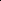
\includegraphics[width=0.8\textwidth]{chemin/vers/capture.png}
    \caption{Vérification du démarrage et de l'état de santé du conteneur Docker}
    \label{fig:docker_startup}
\end{figure}

\section{Option B : Exécution Locale via le Maven Wrapper}
Pour les postes de travail disposant d'un environnement Java 21 natif :
\begin{lstlisting}[language=bash, caption={Exécution native en local sans Docker}]
# Sous Windows PowerShell :
$env:JAVA_HOME = "C:\Program Files\JetBrains\IntelliJ IDEA 2025.3\jbr"
.\mvnw.cmd spring-boot:run

# Sous Linux / macOS :
chmod +x mvnw
./mvnw spring-boot:run
\end{lstlisting}

% ==============================================================================
% CHAPITRE 5 : DÉMONSTRATION DES FONCTIONNALITÉS CLÉS
% ==============================================================================
\chapter{Démonstration des Fonctionnalités Clés}

\section{1. Initialisation de la Root CA Auto-Signée}
Dès le premier lancement, la classe \texttt{CaService} vérifie la présence d'une autorité active en base de données. En cas d'absence, elle initialise la Root CA par défaut :
\begin{itemize}
    \item \textbf{Distinguished Name (DN) :} \texttt{CN=CCN Root CA, OU=Laboratoire Securite, O=ENSET Mohammedia, C=MA}
    \item \textbf{Clé Privée / Publique :} RSA 4096 bits générée par \texttt{SecureRandom}.
    \item \textbf{Période de Validité :} 10 années avec décalage de 24h sur \texttt{notBefore} pour prémunir les dérives d'horloge (\textit{Clock Skew}).
\end{itemize}

\begin{figure}[H]
    \centering
    % TODO : Ajouter la capture d'écran ici
    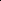
\includegraphics[width=0.8\textwidth]{chemin/vers/capture.png}
    \caption{Interface de gestion et spécifications du certificat de l'Autorité Racine}
    \label{fig:root_ca_ui}
\end{figure}

\section{2. Émission d'un Certificat Client / Serveur (Mode Direct)}
Le mode direct permet à la PKI de générer la biclé RSA (2048 bits) et d'émettre le certificat associé. Ce mode est particulièrement adapté à la délivrance de trousseaux complets d'utilisateurs.

\begin{figure}[H]
    \centering
    % TODO : Ajouter la capture d'écran ici
    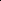
\includegraphics[width=0.8\textwidth]{chemin/vers/capture.png}
    \caption{Formulaire d'émission directe d'un certificat d'entité finale}
    \label{fig:emission_directe}
\end{figure}

À l'issue de l'émission, la plateforme met à disposition trois formats téléchargeables :
\begin{enumerate}
    \item Le certificat public \texttt{.crt} au format X.509 PEM.
    \item La clé privée \texttt{.key} au format PKCS\#8 PEM.
    \item Le conteneur sécurisé chiffré \textbf{PKCS\#12 (\texttt{.p12})} contenant l'ensemble de la chaîne de confiance et la clé privée, directement importable dans les navigateurs ou les magasins de certificats des systèmes d'exploitation.
\end{enumerate}

\section{3. Signature d'une Demande CSR (PKCS\#10)}
Le mode CSR (\textit{Certificate Signing Request}) implémente le paradigme le plus sécurisé dans les architectures réelles : la clé privée ne quitte jamais la machine du client.

Le client génère localement sa biclé et soumet sa demande :
\begin{lstlisting}[language=bash, caption={Génération d'une clé locale et d'une CSR via OpenSSL}]
openssl req -new -newkey rsa:2048 -nodes \
    -keyout client.key -out client.csr \
    -subj "/CN=serveur-web.enset.ma/O=ENSET Mohammedia/C=MA"
\end{lstlisting}

La PKI vérifie la preuve de possession cryptographique (\textit{Proof of Possession}) en validant la signature interne de la CSR avant d'émettre le certificat d'entité finale signé par la Root CA.

\begin{figure}[H]
    \centering
    % TODO : Ajouter la capture d'écran ici
    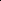
\includegraphics[width=0.8\textwidth]{chemin/vers/capture.png}
    \caption{Soumission et signature d'une CSR PKCS\#10 dans CCN\_PKI}
    \label{fig:signature_csr}
\end{figure}

\section{4. Révocation de Certificat et Émission de la CRL v2}
La révocation permet d'invalider prématurément un certificat dont la clé aurait été compromise, ou dont les attributs d'appartenance auraient changé.

\subsection{Motifs Standardisés RFC 5280}
CCN\_PKI supporte l'ensemble des motifs formels :
\begin{itemize}
    \item \texttt{keyCompromise} (code 1) : La clé privée a été divulguée ou volée.
    \item \texttt{cACompromise} (code 2) : L'autorité de certification a été compromise.
    \item \texttt{affiliationChanged} (code 3) : L'étudiant ou le serveur a changé d'entité.
    \item \texttt{superseded} (code 4) : Remplacé par un certificat plus récent.
    \item \texttt{cessationOfOperation} (code 5) : Le service n'est plus en exploitation.
    \item \texttt{certificateHold} (code 6) : Suspension temporaire réversible.
\end{itemize}

\begin{figure}[H]
    \centering
    % TODO : Ajouter la capture d'écran ici
    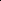
\includegraphics[width=0.8\textwidth]{chemin/vers/capture.png}
    \caption{Modal de confirmation de révocation avec sélection du motif RFC 5280}
    \label{fig:modal_revocation}
\end{figure}

\subsection{Publication Dynamique de la CRL v2}
Dès qu'une révocation est actée, la classe \texttt{CrlService} déclenche la regénération immédiate de la CRL X.509 v2 :
\begin{itemize}
    \item Incrémentation séquentielle du champ \texttt{CRLNumber} (ex: CRL \#1 $\rightarrow$ \#2).
    \item Actualisation des horodatages \texttt{thisUpdate} et \texttt{nextUpdate}.
    \item Signature de la liste avec la clé privée de la Root CA (\texttt{SHA256withRSA}).
    \item Mise à disposition de la CRL aux formats PEM (\texttt{crl.pem}) et DER (\texttt{crl.crl}) sur le point de distribution officiel : \texttt{/api/pki/crl/download}.
\end{itemize}

\begin{figure}[H]
    \centering
    % TODO : Ajouter la capture d'écran ici
    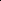
\includegraphics[width=0.8\textwidth]{chemin/vers/capture.png}
    \caption{Tableau de bord de publication de la Liste de Révocation (CRL v2)}
    \label{fig:crl_dashboard}
\end{figure}

\section{5. Moteur de Validation Cryptographique Interne}
L'interface de validation (\texttt{/validate}) implémente un audit automatisé à quatre étapes :
\begin{enumerate}
    \item \textbf{Contrôle de Syntaxe :} Décodage X.509 et parsing des structures ASN.1.
    \item \textbf{Contrôle Temporel :} Vérification que $\text{notBefore} \le t_{\text{actuel}} \le \text{notAfter}$.
    \item \textbf{Vérification Mathématique de la Signature :} Déchiffrement de la signature par la clé publique de la Root CA et comparaison avec l'empreinte SHA-256 recalculée.
    \item \textbf{Contrôle de Révocation :} Vérification de l'absence du numéro de série dans la CRL active.
\end{enumerate}

\begin{figure}[H]
    \centering
    % TODO : Ajouter la capture d'écran ici
    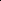
\includegraphics[width=0.8\textwidth]{chemin/vers/capture.png}
    \caption{Rapport de validation d'un certificat actif et conforme}
    \label{fig:validation_active}
\end{figure}

\begin{figure}[H]
    \centering
    % TODO : Ajouter la capture d'écran ici
    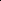
\includegraphics[width=0.8\textwidth]{chemin/vers/capture.png}
    \caption{Détection immédiate d'un certificat révoqué avec cause de compromission}
    \label{fig:validation_revoked}
\end{figure}

\section{6. Vérification Externe Certifiée avec OpenSSL CLI}
Afin de démontrer l'interopérabilité totale de CCN\_PKI avec les standards mondiaux de l'industrie, nous avons testé nos certificats et notre CRL avec l'outil de référence \textbf{OpenSSL 3.x}.

\subsection{Cas A : Vérification d'un Certificat Actif}
\begin{lstlisting}[language=bash, caption={Vérification avec contrôle CRL sous OpenSSL}]
openssl verify -CAfile pki-data/ca/rootCA.pem \
               -CRLfile pki-data/crl/crl.pem \
               -crl_check pki-data/certs/AB28099296E0C67B.crt
\end{lstlisting}

\noindent \textbf{Résultat OpenSSL obtenu :}
\begin{lstlisting}[backgroundcolor=\color{black}, basicstyle=\ttfamily\color{green}\footnotesize]
pki-data/certs/AB28099296E0C67B.crt: OK
\end{lstlisting}

\subsection{Cas B : Vérification d'un Certificat Révoqué}
Après révocation du certificat dans l'interface, la même commande est réexécutée :
\begin{lstlisting}[language=bash, caption={Détection de la révocation par OpenSSL CLI}]
openssl verify -CAfile pki-data/ca/rootCA.pem \
               -CRLfile pki-data/crl/crl.pem \
               -crl_check pki-data/certs/AB28099296E0C67B.crt
\end{lstlisting}

\noindent \textbf{Résultat OpenSSL obtenu :}
\begin{lstlisting}[backgroundcolor=\color{black}, basicstyle=\ttfamily\color{red}\footnotesize]
CN=etudiant.enset.ma, O=ENSET Mohammedia, OU=CyberSec, C=MA
error 23 at 0 depth lookup: certificate revoked
error pki-data/certs/AB28099296E0C67B.crt: verification failed
\end{lstlisting}

\begin{infobox}[title=Interprétation du Code d'Erreur 23 OpenSSL]
Le code de retour \texttt{error 23} correspond rigoureusement à la constante canonique \texttt{X509\_V\_ERR\_CERT\_REVOKED} d'OpenSSL. Cela démontre scientifiquement que notre CRL X.509 v2 est parfaitement formée, encodée et signée selon la RFC 5280.
\end{infobox}

\begin{figure}[H]
    \centering
    % TODO : Ajouter la capture d'écran ici
    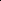
\includegraphics[width=0.8\textwidth]{chemin/vers/capture.png}
    \caption{Exécution et journalisation en direct des commandes d'audit OpenSSL}
    \label{fig:openssl_guide_ui}
\end{figure}

% ==============================================================================
% CHAPITRE 6 : SCÉNARIO RÉALISTE ET CAS DE TESTS DU CAHIER DE RECETTE
% ==============================================================================
\chapter{Scénario Réaliste et Cas de Tests : « Incident de Sécurité sur le Portail ENSET »}

\section{Mise en Situation et Contexte Opérationnel}
Afin d'éprouver la robustesse de notre implémentation \textbf{CCN\_PKI} dans des conditions réelles de cyber-sécurité, nous avons déployé un scénario d'incident complet modélisant la protection des serveurs de recherche du campus de l'\textbf{ENSET Mohammedia}.

\begin{itemize}
    \item \textbf{Le Contexte d'Entreprise :} L'ENSET exige une authentification mutuelle forte (\textit{mTLS}) par certificat X.509 pour accéder aux infrastructures critiques et aux données de recherche.
    \item \textbf{Les Acteurs :}
    \begin{itemize}
        \item \textbf{L'Autorité Centrale :} Le Laboratoire Sécurité de l'ENSET (\texttt{CCN Root CA}).
        \item \textbf{L'Utilisateur :} \textbf{Yassine El Amrani}, étudiant-chercheur en Master Cyber-Sécurité.
        \item \textbf{L'Incident :} Yassine égare une clé USB non chiffrée contenant son certificat et sa clé privée dans un lieu public.
        \item \textbf{L'Équipe SOC / PKI :} L'administrateur de confiance chargé d'interrompre l'attaque et d'émettre la preuve d'audit.
    \end{itemize}
\end{itemize}

\section{Cas de Test 1 : Déploiement et Audit Préalable de l'Autorité Racine}
\textbf{Objectif :} Valider l'intégrité et la conformité normative de l'Autorité Racine avant tout enrôlement d'utilisateurs.

\begin{enumerate}
    \item \textbf{Procédure :} Connexion au tableau de bord \texttt{http://localhost:8080/ca}.
    \item \textbf{Constatations :} 
    \begin{itemize}
        \item Identité de l'autorité : \texttt{CN=CCN Root CA, OU=Laboratoire Securite, O=ENSET Mohammedia, C=MA}.
        \item Puissance cryptographique : Clé asymétrique RSA de 4096 bits.
        \item Extension critique indispensable : \texttt{BasicConstraints: cA=TRUE, pathLenConstraint=unlimited}.
        \item Export du certificat public \texttt{rootCA.crt} au format PEM pour déploiement dans le magasin de confiance des passerelles d'accès.
    \end{itemize}
\end{enumerate}

\begin{figure}[H]
    \centering
    % TODO : Ajouter la capture d'écran ici
    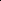
\includegraphics[width=0.8\textwidth]{chemin/vers/capture.png}
    \caption{Cas de Test 1 -- Consultation de l'Autorité Racine CCN\_PKI (RSA 4096)}
    \label{fig:test1_root_ca}
\end{figure}

\section{Cas de Test 2 : Enrôlement de l'Étudiant et Émission du Badge Numérique}
\textbf{Objectif :} Délivrer le badge numérique d'accès avec profils d'extensions mTLS et export sécurisé.

\begin{enumerate}
    \item \textbf{Procédure :} Renseignement du formulaire d'émission directe (\texttt{/issue}) avec le Common Name \texttt{yassine.elamrani@enset-media.ac.ma}, rôle Client/mTLS, et ajout des Subject Alternative Names (SAN) \texttt{DNS:yassine.laptop.enset.ma} et \texttt{IP:192.168.1.45}.
    \item \textbf{Constatations :} 
    \begin{itemize}
        \item Génération automatique de la biclé RSA 2048 bits par la PKI.
        \item Attribution d'un numéro de série cryptographique unique (ex: \texttt{0x5A4C...}).
        \item Mise à disposition de l'archive PKCS\#12 chiffrée (\texttt{.p12}) contenant le certificat et la clé privée pour installation dans le navigateur de l'étudiant.
    \end{itemize}
\end{enumerate}

\begin{figure}[H]
    \centering
    % TODO : Ajouter la capture d'écran ici
    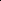
\includegraphics[width=0.8\textwidth]{chemin/vers/capture.png}
    \caption{Cas de Test 2 -- Émission du certificat d'entité finale pour Yassine El Amrani}
    \label{fig:test2_emission_yassine}
\end{figure}

\section{Cas de Test 3 : Contrôle de Fonctionnement Nominal (Accès Autorisé)}
\textbf{Objectif :} Valider que le certificat émis franchit avec succès l'ensemble des règles de validation cryptographique.

\begin{enumerate}
    \item \textbf{Procédure :} Injection du certificat de Yassine dans le moteur d'audit (\texttt{/validate}).
    \item \textbf{Constatations :} 
    \begin{itemize}
        \item Syntaxe ASN.1 : Conforme.
        \item Validité temporelle : Horodatage valide ($\text{notBefore} < \text{Now} < \text{notAfter}$).
        \item Signature CA : Intègre et mathématiquement vérifiée par la clé publique de la Root CA.
        \item Statut CRL : Certificat absent de la liste des révoqués.
        \item Verdict affiché : \textbf{« CERTIFICAT VALIDE »} (Bordure verte et accès au réseau accordé).
    \end{itemize}
\end{enumerate}

\begin{figure}[H]
    \centering
    % TODO : Ajouter la capture d'écran ici
    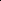
\includegraphics[width=0.8\textwidth]{chemin/vers/capture.png}
    \caption{Cas de Test 3 -- Validation réussie du certificat actif dans le moteur d'audit}
    \label{fig:test3_validation_nominale}
\end{figure}

\section{Cas de Test 4 : Déclaration d'Incident et Révocation d'Urgence (keyCompromise)}
\textbf{Objectif :} Invalider immédiatement le certificat dès notification de la perte de la clé USB.

\begin{enumerate}
    \item \textbf{Procédure :} L'administrateur accède au registre des certificats (\texttt{/certificates}), clique sur « Révoquer » en face de l'entrée de Yassine, et sélectionne formellement le motif standardisé RFC 5280 : \texttt{keyCompromise (Code 1)}.
    \item \textbf{Constatations :} 
    \begin{itemize}
        \item Le statut de l'enregistrement passe instantanément à l'état \texttt{REVOKED}.
        \item Déclenchement automatique du service \texttt{CrlService} : la CRL X.509 v2 est regénérée, son numéro séquentiel (\texttt{CRLNumber}) est incrémenté, et elle est re-signée avec la clé privée de l'autorité.
        \item Publication sur le point de distribution HTTP : \texttt{/api/pki/crl/download}.
    \end{itemize}
\end{enumerate}

\begin{figure}[H]
    \centering
    % TODO : Ajouter la capture d'écran ici
    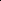
\includegraphics[width=0.8\textwidth]{chemin/vers/capture.png}
    \caption{Cas de Test 4 -- Révocation d'urgence pour motif keyCompromise et publication CRL}
    \label{fig:test4_revocation_crl}
\end{figure}

\section{Cas de Test 5 : Tentative d'Usurpation d'Identité et Détection Immédiate}
\textbf{Objectif :} Simuler une attaque par un tiers malveillant ayant récupéré la clé USB et tentant d'accéder au portail.

\begin{enumerate}
    \item \textbf{Procédure :} Soumission du même certificat dans le moteur de validation.
    \item \textbf{Constatations :} 
    \begin{itemize}
        \item Bien que la signature mathématique de la Root CA soit valide et que la date n'ait pas expiré, le module de contrôle CRL détecte le numéro de série de Yassine dans la nouvelle CRL active.
        \item Verdict affiché : \textbf{« CERTIFICAT RÉVOQUÉ »} (Bordure rouge vif, alerte de sécurité déclenchée, motif de compromission consigné).
        \item L'usurpation d'identité est neutralisée en temps réel.
    \end{itemize}
\end{enumerate}

\begin{figure}[H]
    \centering
    % TODO : Ajouter la capture d'écran ici
    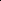
\includegraphics[width=0.8\textwidth]{chemin/vers/capture.png}
    \caption{Cas de Test 5 -- Blocage immédiat de la tentative d'accès par certificat révoqué}
    \label{fig:test5_tentative_usurpation}
\end{figure}

\section{Cas de Test 6 : Preuve d'Audit Judiciaire sous OpenSSL CLI (Erreur 23)}
\textbf{Objectif :} Établir une preuve technique irréfutable et interopérable avec l'outil de référence mondial OpenSSL.

\begin{enumerate}
    \item \textbf{Procédure :} Exécution de l'audit externe via l'interface interactive OpenSSL (\texttt{/openssl-guide}).
    \item \textbf{Commande Exécutée :}
    \begin{lstlisting}[language=bash]
openssl verify -CAfile /app/pki-data/ca/rootCA.pem \
               -CRLfile /app/pki-data/crl/crl.pem \
               -crl_check /app/pki-data/certs/yassine.crt
    \end{lstlisting}
    \item \textbf{Résultat OpenSSL Constaté :}
    \begin{lstlisting}[backgroundcolor=\color{black}, basicstyle=\ttfamily\color{red}\footnotesize]
error 23 at 0 depth lookup: certificate revoked
error /app/pki-data/certs/yassine.crt: verification failed
    \end{lstlisting}
    \item \textbf{Analyse Normative :} Le code d'erreur canonique \textbf{23} confirme que la CRL générée par CCN\_PKI est pleinement conforme à la syntaxe ASN.1 de la RFC 5280.
\end{enumerate}

\begin{figure}[H]
    \centering
    % TODO : Ajouter la capture d'écran ici
    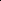
\includegraphics[width=0.8\textwidth]{chemin/vers/capture.png}
    \caption{Cas de Test 6 -- Rapport d'audit OpenSSL CLI attestant l'erreur 23 de révocation}
    \label{fig:test6_audit_openssl}
\end{figure}

\section{Cas de Test 7 : Remédiation Post-Incident et Réémission par Demande CSR}
\textbf{Objectif :} Rétablir l'accès légitime de Yassine en appliquant les bonnes pratiques de sécurité : la clé privée ne doit jamais transiter par le réseau ni être connue de la PKI.

\begin{enumerate}
    \item \textbf{Génération Locale :} Yassine génère une nouvelle paire de clés RSA 2048 bits sur sa station de travail personnelle sécurisée, puis confectionne une demande CSR (PKCS\#10).
    \item \textbf{Soumission :} Envoi de la CSR via l'onglet « Signer CSR » (\texttt{/issue}).
    \item \textbf{Validation Cryptographique :} La PKI vérifie la signature interne de la CSR (\textit{Proof of Possession}), extrait la clé publique du demandeur et émet un nouveau certificat avec un nouveau numéro de série.
    \item \textbf{Bilan :} L'accès est rétabli sans qu'à aucun moment la clé privée de l'étudiant n'ait quitté sa machine.
\end{enumerate}

\begin{figure}[H]
    \centering
    % TODO : Ajouter la capture d'écran ici
    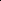
\includegraphics[width=0.8\textwidth]{chemin/vers/capture.png}
    \caption{Cas de Test 7 -- Procédure de remédiation par signature CSR (PKCS\#10)}
    \label{fig:test7_remediation_csr}
\end{figure}

% ==============================================================================
% CHAPITRE 7 : ANALYSE ET REVUE DÉTAILLÉE DU CODE SOURCE
% ==============================================================================
\chapter{Analyse et Revue Détaillée du Code Source}

Cette section examine l'implémentation algorithmique des services fondateurs de \textbf{CCN\_PKI}, illustrée par les extraits de code source commentés et les captures d'écran de l'environnement de développement intégré (IDE).

\section{1. Service de l'Autorité Racine : \texttt{CaService.java}}
La classe \texttt{CaService} assure l'initialisation et la pérennité de l'autorité suprême de certification. Elle instancie un générateur de nombres pseudo-aléatoires sécurisé (\texttt{SecureRandom}), produit la biclé RSA de 4096 bits, et configure le constructeur X.509 v3 auto-signé avec les extensions critiques \texttt{BasicConstraints} et \texttt{KeyUsage}.

\begin{lstlisting}[language=Java, caption={Extrait de CaService.java : Initialisation de la Root CA}]
// Generation de la bicle RSA 4096 bits
KeyPairGenerator keyGen = KeyPairGenerator.getInstance("RSA", "BC");
keyGen.initialize(4096, new SecureRandom());
KeyPair caKeyPair = keyGen.generateKeyPair();

// Construction du certificat auto-signe X.509 v3
X500Name issuer = new X500Name("CN=CCN Root CA, OU=Laboratoire Securite, O=ENSET Mohammedia, C=MA");
BigInteger serial = new BigInteger(64, new SecureRandom());
Date notBefore = new Date(System.currentTimeMillis() - 24 * 3600 * 1000L); // Tolerance clock-skew
Date notAfter = new Date(System.currentTimeMillis() + 10L * 365 * 24 * 3600 * 1000L);

JcaX509v3CertificateBuilder certBuilder = new JcaX509v3CertificateBuilder(
    issuer, serial, notBefore, notAfter, issuer, caKeyPair.getPublic());

// Extensions RFC 5280 obligatoires pour une Autorite Racine
certBuilder.addExtension(Extension.basicConstraints, true, new BasicConstraints(true));
certBuilder.addExtension(Extension.keyUsage, true, new KeyUsage(
    KeyUsage.keyCertSign | KeyUsage.cRLSign | KeyUsage.digitalSignature));
\end{lstlisting}

\begin{figure}[H]
    \centering
    % TODO : Ajouter la capture d'écran ici
    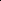
\includegraphics[width=0.8\textwidth]{chemin/vers/capture.png}
    \caption{Code source de CaService.java dans l'environnement de développement}
    \label{fig:code_ca_service}
\end{figure}

\section{2. Service d'Émission et Signature CSR : \texttt{CertificateIssuingService.java}}
Ce service prend en charge deux flux distincts : l'émission directe avec fourniture de clés et la signature externe de demandes de certificats PKCS\#10. 

Dans le cas d'une demande CSR, la PKI valide préalablement la signature mathématique contenue dans la requête pour attester que le client détient bien la clé privée correspondant à la clé publique transmise (\textit{Proof of Possession}), avant d'y greffer les extensions de politique (KeyUsage, EKU, SAN, CDP).

\begin{lstlisting}[language=Java, caption={Extrait de CertificateIssuingService.java : Validation et Signature CSR}]
// Verification cryptographique de la signature interne de la CSR (PKCS#10)
PKCS10CertificationRequest csr = new PKCS10CertificationRequest(csrPemBytes);
ContentVerifierProvider verifier = new JcaContentVerifierProviderBuilder()
    .setProvider("BC").build(csr.getSubjectPublicKeyInfo());

if (!csr.isSignatureValid(verifier)) {
    throw new IllegalArgumentException("Signature CSR invalide: echec de la preuve de possession");
}

// Extraction de la cle publique cliente et construction du certificat X.509 v3
X509v3CertificateBuilder certBuilder = new X509v3CertificateBuilder(
    caCertificateHolder.getSubject(),
    new BigInteger(64, new SecureRandom()),
    notBefore, notAfter,
    csr.getSubject(),
    csr.getSubjectPublicKeyInfo()
);

// Ajout de l'extension BasicConstraints cA=FALSE avec criticite active
certBuilder.addExtension(Extension.basicConstraints, true, new BasicConstraints(false));
\end{lstlisting}

\begin{figure}[H]
    \centering
    % TODO : Ajouter la capture d'écran ici
    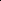
\includegraphics[width=0.8\textwidth]{chemin/vers/capture.png}
    \caption{Code source de CertificateIssuingService.java dans l'IDE}
    \label{fig:code_issuing_service}
\end{figure}

\section{3. Service de Révocation et Génération CRL v2 : \texttt{CrlService.java}}
Conformément à la RFC 5280, la classe \texttt{CrlService} instancie le constructeur \texttt{X509v2CRLBuilder}. Chaque certificat révoqué est consigné avec son numéro de série, sa date de révocation et son extension individuelle \texttt{ReasonCode} (\texttt{CRLReason}). La liste globale reçoit un identifiant incrémental (\texttt{CRLNumber}) et l'empreinte de la clé émettrice (\texttt{AuthorityKeyIdentifier}).

\begin{lstlisting}[language=Java, caption={Extrait de CrlService.java : Signature de la CRL v2 selon la RFC 5280}]
X509v2CRLBuilder crlBuilder = new X509v2CRLBuilder(caCertHolder.getSubject(), thisUpdate);
crlBuilder.setNextUpdate(nextUpdate);

// Ajout de chaque certificat revoque avec son motif specifique
for (CertificateEntity cert : revokedList) {
    BigInteger serial = new BigInteger(cert.getSerialNumberHex(), 16);
    ExtensionsGenerator extGen = new ExtensionsGenerator();
    extGen.addExtension(Extension.reasonCode, false, 
        CRLReason.lookup(cert.getRevocationReasonCode()));
    crlBuilder.addCRLEntry(serial, cert.getRevokedAt(), extGen.generate());
}

// Ajout du numero sequentiel de CRL (CRLNumber)
crlBuilder.addExtension(Extension.cRLNumber, false, new CRLNumber(BigInteger.valueOf(crlSeqNumber)));

// Signature avec la cle privee de la Root CA
ContentSigner signer = new JcaContentSignerBuilder("SHA256withRSA").setProvider("BC").build(caPrivateKey);
X509CRLHolder crlHolder = crlBuilder.build(signer);
\end{lstlisting}

\begin{figure}[H]
    \centering
    % TODO : Ajouter la capture d'écran ici
    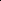
\includegraphics[width=0.8\textwidth]{chemin/vers/capture.png}
    \caption{Code source de CrlService.java dans l'environnement de développement}
    \label{fig:code_crl_service}
\end{figure}

\section{4. Moteur de Validation Cryptographique : \texttt{ValidationService.java}}
Le validateur exécute un audit rigoureux en cascade, combinant vérification d'encodage, bornes d'horloge, validation de la signature asymétrique de l'autorité émettrice et consultation de la liste des certificats révoqués.

\begin{lstlisting}[language=Java, caption={Extrait de ValidationService.java : Audit 4 Niveaux}]
// 1. Controle temporel
cert.checkValidity(new Date());

// 2. Verification mathematique de la signature de la Root CA
cert.verify(caCert.getPublicKey(), "BC");

// 3. Controle du statut dans la CRL active
X509CRLEntry entry = crl.getRevokedCertificate(cert.getSerialNumber());
if (entry != null) {
    return ValidationResult.revoked(entry.getRevocationDate(), entry.getRevocationReason());
}

return ValidationResult.valid("Certificat conforme et pleinement valide.");
\end{lstlisting}

\begin{figure}[H]
    \centering
    % TODO : Ajouter la capture d'écran ici
    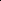
\includegraphics[width=0.8\textwidth]{chemin/vers/capture.png}
    \caption{Code source de ValidationService.java dans l'IDE}
    \label{fig:code_validation_service}
\end{figure}

\section{5. Infrastructure Docker Multi-Stage et Persistance}
L'infrastructure de conteneurisation garantit une chaîne de compilation indépendante de la machine hôte. Le stage de compilation compile l'application sous Alpine JDK 21, tandis que le runtime finalise l'image avec OpenSSL et cURL pour les tests d'interopérabilité.

\begin{lstlisting}[language=docker, caption={Dockerfile multi-stage du projet CCN\_PKI}]
# Stage 1: Build applicatif Maven
FROM eclipse-temurin:21-jdk-alpine AS builder
WORKDIR /build
COPY .mvn/ .mvn/
COPY mvnw pom.xml ./
RUN ./mvnw dependency:go-offline -B
COPY src/ src/
RUN ./mvnw clean package -DskipTests

# Stage 2: Runtime securise et leger
FROM eclipse-temurin:21-jre-alpine
RUN apk add --no-cache openssl curl bash tzdata
WORKDIR /app
COPY --from=builder /build/target/CCN_PKI-*.jar app.jar
EXPOSE 8080
VOLUME ["/app/pki-data"]
ENTRYPOINT ["java", "-jar", "app.jar"]
\end{lstlisting}

\begin{figure}[H]
    \centering
    % TODO : Ajouter la capture d'écran ici
    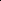
\includegraphics[width=0.8\textwidth]{chemin/vers/capture.png}
    \caption{Configuration Dockerfile et docker-compose.yml dans l'éditeur de code}
    \label{fig:code_dockerfile}
\end{figure}

% ==============================================================================
% CHAPITRE 8 : RÉFÉRENTIEL DES API REST
% ==============================================================================
\chapter{Référentiel des API REST}

L'application expose une interface RESTful complète permettant l'automatisation programmatique des opérations PKI par des scripts ou des agents distants.

\begin{table}[H]
\centering
\small
\begin{tabularx}{\textwidth}{l l X}
\toprule
\textbf{Méthode} & \textbf{Point d'Accès (Endpoint)} & \textbf{Description et Paramètres} \\
\midrule
\texttt{GET} & \texttt{/api/pki/status} & Retourne les métriques, l'état de la CA et de la CRL en JSON. \\
\addlinespace
\texttt{POST} & \texttt{/api/pki/ca/init} & Initialise ou régénère l'Autorité Racine auto-signée. \\
\addlinespace
\texttt{GET} & \texttt{/api/pki/ca/cert?format=pem|der} & Télécharge le certificat public de la Root CA. \\
\addlinespace
\texttt{POST} & \texttt{/api/pki/certificates/issue} & Émet un certificat avec génération automatique de la biclé. \\
\addlinespace
\texttt{POST} & \texttt{/api/pki/certificates/issue-csr} & Signe une demande de certificat CSR (PKCS\#10). \\
\addlinespace
\texttt{GET} & \texttt{/api/pki/certificates} & Retourne la liste JSON complète des certificats enregistrés. \\
\addlinespace
\texttt{GET} & \texttt{/api/pki/certificates/\{serial\}/cert} & Télécharge le certificat client/serveur au format \texttt{.crt}. \\
\addlinespace
\texttt{GET} & \texttt{/api/pki/certificates/\{serial\}/key} & Télécharge la clé privée associée (si émis en mode direct). \\
\addlinespace
\texttt{GET} & \texttt{/api/pki/certificates/\{serial\}/p12} & Télécharge l'archive PKCS\#12 protégée par mot de passe. \\
\addlinespace
\texttt{POST} & \texttt{/api/pki/certificates/revoke} & Révoque un certificat actif et publie la nouvelle CRL. \\
\addlinespace
\texttt{GET} & \texttt{/api/pki/crl/download?format=pem|der} & Point de distribution officiel de la CRL v2 (RFC 5280). \\
\addlinespace
\texttt{POST} & \texttt{/api/pki/certificates/validate} & Soumet un certificat PEM pour analyse et rapport de conformité. \\
\bottomrule
\end{tabularx}
\caption{Documentation des points de terminaison de l'API REST de CCN\_PKI}
\label{tab:api_endpoints}
\end{table}

% ==============================================================================
% CHAPITRE 9 : ANALYSE CRITIQUE (FORCES, LIMITES ET PERSPECTIVES)
% ==============================================================================
\chapter{Analyse Critique (Forces, Limites et Perspectives)}

Conformément aux directives de l'ENSET Mohammedia valorisant le recul réflexif sur les architectures de confiance, cette section dresse le bilan critique de notre MVP.

\section{Points Forts et Réussites de la Solution}
\begin{enumerate}
    \item \textbf{Rigueur Normative :} Respect scrupuleux des spécifications RFC 5280 (criticité des extensions, gestion des SAN, formats d'horodatage UTC/GeneralizedTime).
    \item \textbf{Dualité d'Émission :} Capacités complètes en mode centralisé direct et en mode décentralisé CSR (PKCS\#10), garantissant le respect de la confidentialité des clés clientes.
    \item \textbf{Double Niveau d'Audit :} Intégration d'un validateur interne exhaustif complété par une compatibilité certifiée avec l'outil international OpenSSL.
    \item \textbf{Conteneurisation Optimisée :} Déploiement propre et immédiat via Docker Compose sous architecture Alpine Linux sécurisée.
    \item \textbf{Expérience Utilisateur :} Interface Web ergonomique facilitant la visualisation instantanée des empreintes et l'exportation des certificats.
\end{enumerate}

\section{Limites Identifiées du MVP}
\begin{enumerate}
    \item \textbf{Architecture Monocouche (Mono-niveau) :} CCN\_PKI met en œuvre une Root CA unique qui émet directement les certificats d'entité finale. Dans une infrastructure d'entreprise réelle, la Root CA est conservée hors-ligne (\textit{Offline Root CA}) pour prévenir toute compromission fatale, et délègue l'émission quotidienne à une ou plusieurs autorités subordonnées (\textit{Intermediate / Issuing CAs}).
    \item \textbf{Absence du Protocole OCSP (RFC 6960) :} La gestion des révocations s'appuie exclusivement sur les listes CRL. Lorsque le volume de certificats révoqués devient conséquent, le téléchargement intégral et périodique de la CRL entraîne une surcharge de bande passante que le protocole OCSP (\textit{Online Certificate Status Protocol}) résout par des requêtes légères en temps réel.
    \item \textbf{Stockage Logiciel des Clés :} Les clés privées sont persistées sous forme chiffrée sur le système de fichiers, sans adossement à un composant matériel cryptographique certifié de type \textbf{HSM} (\textit{Hardware Security Module}).
\end{enumerate}

\section{Perspectives et Pistes d'Évolution}
\begin{itemize}
    \item \textbf{Implémentation d'un Répondeur OCSP :} Ajout d'un point d'accès \texttt{/api/pki/ocsp} permettant l'interrogation granulaire et signée du statut d'un certificat à la volée.
    \item \textbf{Automatisation par Protocole ACME (RFC 8555) :} Déploiement d'un agent ACME (analogue à l'architecture Let's Encrypt) pour le renouvellement automatisé sans intervention humaine.
    \item \textbf{Hiérarchie à Deux Niveaux :} Séparation architecturale formelle entre Root CA (auto-signée, durée 15 ans) et Intermediate CA (durée 3 ans).
\end{itemize}

% ==============================================================================
% CONCLUSION ET BIBLIOGRAPHIE
% ==============================================================================
\chapter*{Conclusion Générale}
\addcontentsline{toc}{chapter}{Conclusion Générale}

Le développement du projet \textbf{CCN\_PKI} a permis à notre groupe de matérialiser concrètement les concepts théoriques fondamentaux abordés durant le cours de \textit{Confiance Numérique et Accès Biométrique}. 

En partant d'une feuille blanche, nous avons conçu et implémenté une autorité de certification robuste et pleinement interopérable avec les standards mondiaux de l'IETF et la suite logicielle OpenSSL. De la génération des clés RSA à la gestion fine des extensions critiques, en passant par le cycle de révocation dynamique via CRL v2 et la conteneurisation Docker, ce travail pratique nous a conféré une maîtrise technique et opérationnelle des architectures de sécurité à clés publiques, indispensables à notre futur profil d'ingénieurs en cyber-sécurité.

% ------------------------------------------------------------------------------
% BIBLIOGRAPHIE & NORMES OFFICIELLES
% ------------------------------------------------------------------------------
\begin{thebibliography}{99}
\addcontentsline{toc}{chapter}{Références et Normes}

\bibitem{rfc5280}
D. Cooper, S. Santesson, S. Farrell, S. Boeyen, R. Housley, W. Polk.
\textit{Internet X.509 Public Key Infrastructure Certificate and Certificate Revocation List (CRL) Profile}.
RFC 5280, IETF Standards Track, Mai 2008.

\bibitem{rfc2986}
M. Nystrom, B. Kaliski.
\textit{PKCS \#10: Certification Request Syntax Specification Version 1.7}.
RFC 2986, Novembre 2000.

\bibitem{rfc6960}
S. Santesson, M. Myers, R. Ankney, A. Malpani, S. Galperin, C. Adams.
\textit{X.509 Internet Public Key Infrastructure Online Certificate Status Protocol - OCSP}.
RFC 6960, Juin 2013.

\bibitem{bouncycastle}
The Legion of the Bouncy Castle.
\textit{Bouncy Castle Cryptography APIs Documentation for Java (Release 1.79)}.
\url{https://www.bouncycastle.org/documentation.html}.

\bibitem{openssl}
The OpenSSL Project.
\textit{OpenSSL Documentation -- Cryptography and SSL/TLS Toolkit (Version 3.x)}.
\url{https://www.openssl.org/docs/}.

\bibitem{springboot}
VMware Tanzu / Spring Team.
\textit{Spring Boot Reference Documentation (Version 3.3.x)}.
\url{https://docs.spring.io/spring-boot/}.

\end{thebibliography}

\end{document}
